\documentclass[a4paper,14pt]{extarticle}

\usepackage[utf8x]{inputenc}
\usepackage[T1,T2A]{fontenc}
\usepackage[russian]{babel}
\usepackage{hyperref}
\usepackage{indentfirst}
\usepackage{here}
\usepackage{array}
\usepackage{graphicx}
\usepackage{caption}
\usepackage{subcaption}
\usepackage{chngcntr}
\usepackage{amsmath}
\usepackage{amssymb}
\usepackage{pgfplots}
\usepackage{pgfplotstable}
\usepackage[left=2cm,right=2cm,top=2cm,bottom=2cm,bindingoffset=0cm]{geometry}
\usepackage{multicol}

\renewcommand{\le}{\ensuremath{\leqslant}}
\renewcommand{\leq}{\ensuremath{\leqslant}}
\renewcommand{\ge}{\ensuremath{\geqslant}}
\renewcommand{\geq}{\ensuremath{\geqslant}}
\renewcommand{\epsilon}{\ensuremath{\varepsilon}}
\renewcommand{\phi}{\ensuremath{\varphi}}

\counterwithin{figure}{section}
\counterwithin{equation}{section}
\counterwithin{table}{section}
\newcommand{\sign}[1][5cm]{\makebox[#1]{\hrulefill}} % Поля подписи и даты
\graphicspath{{pics/}} % Путь до папки с картинками
\captionsetup{justification=centering,margin=1cm}
\def\arraystretch{1.3}

\begin{document}

\begin{titlepage}
\begin{center}
	\textbf{Санкт-Петербургский Политехнический Университет \\Петра Великого}\\[0.3cm]
	\small Институт компьютерных наук и технологий \\[0.3cm]
	\small Кафедра компьютерных систем и программных технологий\\[4cm]
	
	\textbf{ОТЧЕТ}\\ \textbf{о лабораторной работе}\\[0.5cm]
	\textbf{<<Исследование частотных характеристик пассивных RC-цепей>>}\\[0.1cm]
	\textbf{Электротехника и Электроника}\\[10.5cm]
\end{center}

\begin{flushright}
	\begin{minipage}{0.60\textwidth}
		\begin{flushleft}
			\small \textbf{Работу выполнили студенты}\\[3mm]
			\small группа 23501/4 \hspace*{17mm} Дьячков В.В.\\[3mm]
			\small группа 23501/4 \hspace*{17mm} Ламтев А.Ю.\\[5mm]
			
			\small \textbf{Преподаватель}\\[5mm]
		 	\small \sign[3.5cm] \hspace*{8mm} к.т.н., доц. Кочетков Ю.Д.\\[0.5cm]
		\end{flushleft}
	\end{minipage}
\end{flushright}

\vfill

\begin{center}
	\small Санкт-Петербург\\
	\small \the\year
\end{center}
\end{titlepage}

\section{Цель работы}

Cравнение теоретических и экспериментальных характеристик фильтров,
проектирование и настройка фильтров высокого порядка, построенных на
операционных усилителях. 

\section{Чертеж схемы исследуемого устройства}

\begin{figure}[H]
\begin{center}
	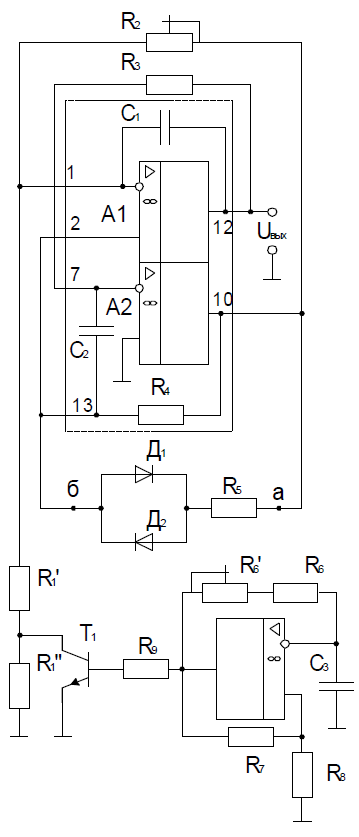
\includegraphics[width=0.45\textwidth]{scheme}
	\caption{Схема управляемого генератора}
\end{center}
\end{figure}

\section{Исходные данные}

\begin{table}[H]
\begin{center}
	\caption{Исходные данные}
	\def\tabcolsep{8pt}
	\begin{tabular}{|c|c|c|c|c|c|c|c|c|c|c|c|c|}
		\hline
		$E{01}$, В &
		$E{02}$, В &
		$f_0$, кГц &
		$R_3$, кОм &
		$R_4$, кОм &
		$R_5$, кОм &
		$R_6$, кОм \\
		\hline
		15 &
		-15 &
		65 &
		33 &
		6.8 &
		24 &
		8.2 \\
	    \hline	
	\end{tabular}
\end{center}
\end{table}

\begin{table}[H]
\begin{center}
	\def\tabcolsep{8pt}
	\begin{tabular}{|c|c|c|c|c|c|c|c|c|c|c|c|c|}
		\hline
		$R_6^*$, кОм &
		$R_7$, кОм &
		$R_8$, кОм &
		$R_9$, кОм &
		$C_1$, нФ &
		$C_2$, нФ \\
		\hline
		1 &
		8.2 &
		3.9 &
		1.3 &
		1 &
		2 \\
	    \hline	
	\end{tabular}
\end{center}
\end{table}

\section{Теоретические расчёты}

\begin{displaymath}
	R_\text{2 min} = \frac{R_4 \cdot C_2}{C_1} = \frac{6.8 \cdot 10^3 \cdot 2 \cdot 10^{-9}}{10^{-9}} = 13.6 \text{ кОм}
\end{displaymath}

\begin{displaymath}
	R_1 = \left((2\pi f_0)^2 R_3 C_1 C_2 \right)^{-1} = \left((2\pi \cdot 6.5 \cdot 10^3)^2 \cdot 33 \cdot 10^3 \cdot 2 \cdot 10^{-9} \cdot 10^{-9} \right)^{-1} = 9 \text{ кОм}
\end{displaymath}

\begin{displaymath}
	C_3 = \frac{16}{f_0 \cdot R_6} = \frac{16}{6.5 \cdot 10^3 \cdot 8.2 \cdot 10^3} = 300 \text{ нФ}
\end{displaymath}

\section{Экспериментально снятые зависимости}

\begin{table}[H]
\begin{center}
	\caption{ЛАЧХ активного RC-фильтра 4 порядка}
	\label{tab:diff-int}
	\def\tabcolsep{20pt}
	\pgfplotstabletypeset[col sep=comma,
	    columns={r,f0},
	    column type/.add={|c|}{},
	    columns/r/.style={fixed, column name={$R_1$, кОм}},
	    columns/f0/.style={fixed, precision=3, zerofill, column name={$f_0$, кГц}},
	    every nth row={1}{before row=\hline},
	    every head row/.style={before row=\hline, after row=\hline},
	    every last row/.style={after row=\hline}
	   ]{data/f0_as_f_of_R_exp.csv}
\end{center}
\end{table}

\begin{figure}[H]
\begin{center}
	\begin{tikzpicture} [every plot/.append style={thick}]
		\begin{axis}[
			height=0.45\textheight,
			width=0.95\textwidth,
			legend pos = north east,
			xlabel={$R_1$, кОм},
			ylabel={$f_0$, кГц},
			axis x line = middle,
			axis y line = left,
			xmode=linear,
			xmin = 0,
			xmax = 120,
			ymin = 0,
			ymax = 13,
			grid=major
		]
		\addplot [smooth, mark=square*, blue] table[x=r,y=f0,col sep=comma]{data/f0_as_f_of_R_exp.csv};
		%\addplot [smooth, mark=square*, blue] table[x=r,y=f0,col sep=comma]{data/f0_as_f_of_R_theory.csv};
		\legend{Эксп., Теор.}
		\end{axis}
	\end{tikzpicture}
	\caption{ЛАЧХ активного RC-фильтра 4 порядка}
	\label{plot:rectifier}
\end{center}
\end{figure}

\section{Погрешности}

\subsection{Предельно допустимые порешности}

\begin{displaymath}
\begin{aligned}
	\delta_{max} f = \delta_{max} Q = \delta_{max} L_m = \sqrt{(\delta R_1)^2 + (\delta R_2)^2 + (\delta C_3)^2 + (\delta C_4)^2} = \\ = \sqrt{0.1^2 + 0.1^2 + 0.1^2 + 0.1^2} = 0.2 = 20\%
\end{aligned}
\end{displaymath}

\begin{displaymath}
	\delta_{max} (\Delta f) = \sqrt{(\delta R_2)^2 + (\delta C_4)^2} = \sqrt{0.1^2 + 0.1^2} = 0.141 = 14.1\%
\end{displaymath}

\subsection{Приведённые погрешности}

\begin{displaymath}
	\delta f_1 = \left|\frac{f_\text{1 теор.} - f_\text{1 эксп.}}{f_\text{1 теор.}} \right| = \left|\frac{500 - 478}{500}\right| = 0.044 = 4.4\% < \delta_{max} f = 20\%
\end{displaymath}



\section{Выводы}

Приведённые погрешности полученных в ходе эксперимента значений $f$, $\Delta f$, $Q$ и $L_m$ не превышают предельно допустимые погрешности.

Таким образом, формулы \ref{eq:4:1} -- \ref{eq:4:4} являются верными.

\end{document}